\chapter*{Remerciements}
Je tiens tout d'abord à remercier l'Université de technologie de Compiègne, le \acrshort{cnes} et CS Group, qui ont su s'entendre pour me permettre de réaliser cette thèse dans de bonnes conditions. J'ai eu la chance de pouvoir travailler entre Compiègne et Toulouse, et d'y rencontrer de nombreuses personnes qui m'ont épaulé durant ces trois années particulièrement enrichissantes. Je tiens ensuite à remercier les membres du jury, notamment M. Luc Jaulin pour avoir suivi mes travaux de thèse depuis nos échanges lors de la journée Imagin. Je remercie également Mme Isabelle Bloch et M. Marc Pierrot Deseilligny pour avoir accepté de rapporter ce travail et pour le temps qu’ils y ont consacré ainsi que pour leurs remarques pertinentes. Je voudrais aussi remercier chaleureusement M. Olivier Strauss, qui a manifesté son intérêt pour mes travaux depuis les premiers instants, m'a permis de découvrir son laboratoire du LIRMM, et a piqué ma curiosité avec des problèmes de traitement d'image auxquels je réfléchis encore aujourd'hui. Un grand merci à M. Benjamin Quost, qui a accepté de présider ce jury, mais aussi de partager son bureau pour que s'y déroulent mes réunions de thèse lorsque j'étais un peu perdu.

Je voudrais remercier Etienne Berthier et Simon Gascoin, pour tout l'intérêt qu'ils ont porté à mes travaux. Mais aussi pour m'avoir généreusement partagé leurs données, et mis en contact avec Liss Marie Andreassen et Brian Menounos qui ont fait de même. C'était pour moi bien plus que de simples données. J'aimerais également remercier Yoann Steux, pour tout le temps passé à résoudre mes problèmes sur \acrshort{cars}.

Bien entendu, merci à Simon, Tatha, Tom, pour avoir égayé mes soirées compiègnoises. Cassandra, Gabriela, Lou, Marion, Alice, Martin, et surtout Camille, pour tout ce qu'on a vécu au CNES, mais aussi en dehors.

Je ne dis pas merci à :
\begin{itemize}
    \item La personne qui m’a dit qu’installer \acrshort{cars} était facile
    \item Mon vélo, et surtout mes freins. Trop de temps et d’efforts passés à le réparer, et encore plus à me réparer moi-même
\end{itemize}

Un grand merci à ma soeur, mes parents et grands-parents, qui se sont intéressés à mes travaux et m’ont toujours souhaité le meilleur. Merci également à mon autre famille, chinoise, pour les déménagements et pour avoir pris soin de mes papilles gustatives. À toi, Virginie, pour m’avoir soutenu, écouté, t’être intéressée à mes travaux quand bien même ce que je racontais n’avait que peu d’intérêt. M’avoir changé les idées quand je voulais vivre autre chose que cette thèse, et avoir accepté que je n’aie parfois pas d’autre vie que celle-ci. J'espère pouvoir te rendre, un jour, tout ce que tu m'as donné.

Un grand merci à Manu, qui a fait la jonction entre ces deux mondes que sont la galaxie CNES et la communauté des probas imprécises. Sans toi, cette thèse n'aurait sûrement pas eu lieu, ou du moins pas sous cette forme. Un grand merci à Loïc, avec le regret de n'avoir pas passé encore plus de temps à travailler à tes côtés. Je t'admirerai toujours pour tes conseils et remarques qui touchent toujours juste. Mais également pour tes commentaires qui m'ont beaucoup fait rire lors de la rédaction de ce manuscrit. Sébastien, bien entendu, je te serai à jamais reconnaissant pour m'avoir guidé, conseillé et épaulé lorsque j'étais perdu dans des concepts théoriques qui me dépassaient. Pour avoir dit ce qui n'allait pas, mais aussi toujours ce qui allait bien. Merci pour m'avoir toujours accordé ton temps, même quand tu ne l'avais pas.

\begin{wrapfigure}{L}{0.2\textwidth}
  \begin{center}
    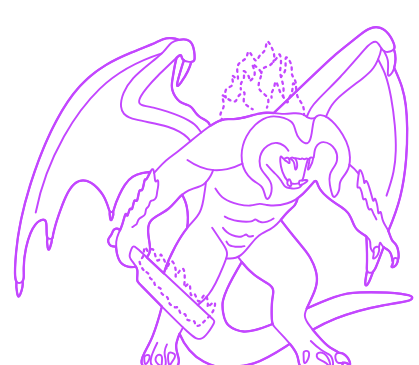
\includegraphics[width=0.2\textwidth]{tmp/balrog.png}
  \end{center}
\end{wrapfigure}
Enfin, un grand merci à Manue, qui m’a convaincu de me lancer dans cette aventure, et qui est restée jusqu’au bout — et même parfois très tard — pour enrichir mon travail de ses idées et de ses conseils. Tu m’as dit au début de ma thèse, que je la commencerai en étant sous ta supervision, et que je la terminerai en étant ton collègue. Plus qu’une collègue, j’ai terminé cette thèse avec un modèle, un guide, une amie. Tu es la flamme d’Udûn qui éclairait les recoins les plus sombres du cluster ou de l’écriture de manuscrit. Chanceux seront les prochains doctorants qui t’auront comme maître Jedi.
\begin{center}
    
\includegraphics[width=0.2\textwidth]{tmp/gandalf.png}
\end{center}
\clearpage